\chapter{The privacy monitoring system}
\label{pivot}
As demonstrated in the previous chapter, although the LoRaWAN protocol is designed to be very secure, some still unsolved privacy issues can compromise the confidentiality of information exchanged within the LoRa network. In this chapter, we introduce \textit{PIVOT}, a LoRaWAN privacy monitoring system that, analyzing the traffic flow, detects any weak endpoint that could expose sensitive information to unauthorized parties. The goal of PIVOT is to strengthen the traffic exchanged between ED and servers to avoid adversaries from conducting privacy-related threats such as malicious fingerprints or information leaks.
\\
The rest of the chapter is structured as follows. First, in Section \ref{goals}, we present the main principle and guidelines used in designing our system. In Section \ref{system}, we deepen PIVOT, going from the assumptions to the definition of the detection algorithm. Finally, we illustrate the core metrics supplied by PIVOT that the operator can use to monitor the network environment and check the current status of devices.
\vspace{5mm}

\section{Design Goals}
\label{goals}
The following are the main points followed for the development of PIVOT.
\begin{enumerate}
	\item \textit {Detection} of vulnerable devices. To avoid the threat described in Section \ref {address_identification}, PIVOT should properly identify that endpoints of the network whose \textit {DevAddr} - \textit {DevEUI} address pair could be discovered by unauthorized listeners.
	\item \textit{Monitoring} the status of end-device. Our system should give the operator a transparent vision of the state of the network, showing, for example, the number of detected devices. 
	\item \textit{Strengthening} of the network. PIVOT should represent an additional security layer for the LoRaWAN protocol to better preserve the confidentiality of the LoRa traffic exchanged between the endpoints and the Network Server.
	\item \textit{Modelling} the behavior of periodic devices. Since EDs that send packets regularly are inclined to threat we are trying to avoid, PIVOT should discover and model their behavior.
	\item \textit{Stream} of data. PIVOT should constantly analyze the traffic. Since it cannot analyze the entire group of messages only once they have all been sent, it has to make a decision every time a single message is exchanged.
	\item \textit{Minimize} the delay. Vulnerable devices need to be detected quickly to leave them exposed as little time as possible.
	\item \textit{Accuracy} of the detection. The detection procedure of PIVOT should be detailed and precise as far as possible. The error rate should be kept low.
	\item \textit{Lightweight}. The system should be designed to have a small memory footprint (RAM usage) and low CPU usage, overall a low usage of system resources.
	\item \textit{Filter} only the necessary data from all network traffic. As we will explain later, not all LoRa messages are relevant to our goal.
	\item \textit{Passivity}. Our system should collect and analyze the packets without interfering with the normal operations of the network.
	\item \textit{Scalability}. PIVOT should be able to scale, working well on both a small data set and a larger one.
\end{enumerate}

\newpage

\section{System Description}
\label{system}
The main policy of PIVOT is to \textit{detect} and \textit{protect} devices in the LoRa network that are vulnerable to information disclosure. In this section, we explain how our system can achieve this.
\vspace{5mm}

\subsection{Assumptions}
The endpoints of the LoRa network in which PIVOT operates should be LoRaWAN v1.1 compliant. If they get disconnected or lose the connection with the Network Server, should try a new activation procedure, which gives them a new DevAddress. Devices should perform exclusively the Over-the-Air Activation (OTAA) to join the network since PIVOT needs to intercept and collect \jr messages used in the activation procedure. This condition results satisfied because LoRaWAN specification recommends using OTAA for security and scalability reasons. 
\\
Another assumption is that these devices should transmit packets periodically. These requirements find evidence in real case studies. For example, the analysis carried out on a LoRaWAN service of an Italian operator \cite{devil} shows up that the majority of devices send 24 packets each hour, the 25th one after 30 seconds, and then repeat the process. We can argue that when a device sends packets periodically, it follows a temporal \textit{pattern}, a behavior repeated continuously over time.
\vspace{5mm}

\subsection{Architecture}
Figure \ref{fig:pivarchitecture} reports the high-level architecture of PIVOT. 
\begin{figure}
    \centering
    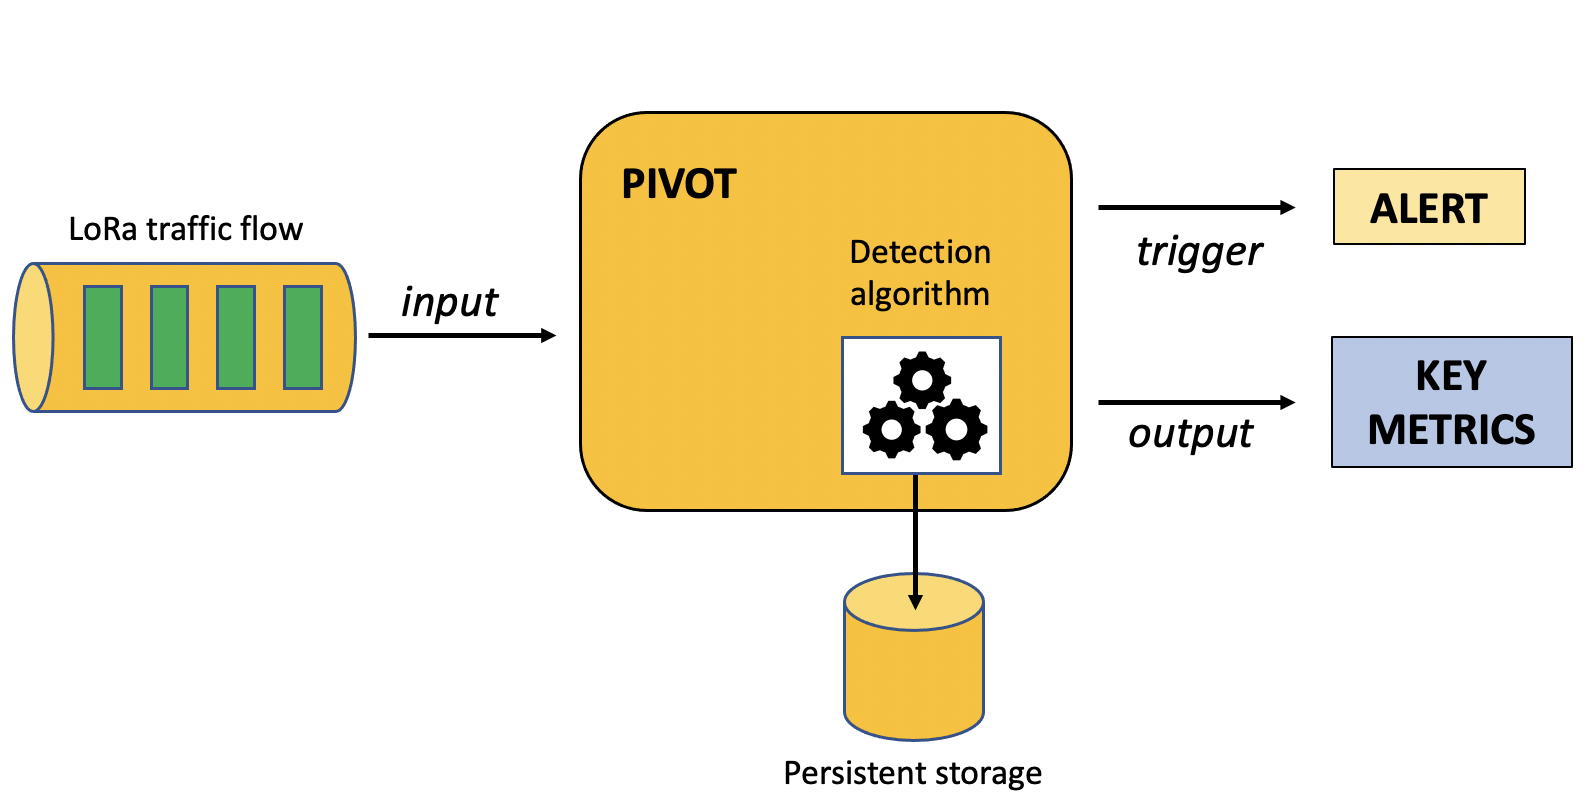
\includegraphics[width=0.7\linewidth]{images/pivot/architecture_detail.png}
    \caption{The architecture of PIVOT}
    \vspace{4ex}%
    \label{fig:pivarchitecture}
\end{figure}
The system passively collects the LoRa stream, filtering \textit{uplink} and \textit{join-request} messages, the only needed for our purpose.
\\
Each elaborated frame represents the input of the so-called \textit{detection} algorithm. This procedure, which is the core of PIVOT, analyzes the incoming messages and tries to deduce if the devices that generated them could be at risk and, in that case, it triggers an alert to the network operator.
\\
During its analysis, the detection algorithm constantly outputs to the operator a set of metrics it can use to check the current network status. They consist of statistical reports about the current number of join/re-joined devices and correlated percentage of vulnerable endpoints that are still operating. In this way, it is possible to check the current level of security of the network and, if needed, execute actions to decrease the level of exposure of vulnerable EDs. 
\\
Finally, PIVOT uses a persistent storage system to store some relevant data used to support the functioning of the detection algorithm.

\vspace{5mm}

From a technical point of view, this algorithm belongs to the streaming algorithms family, which main characteristics are:
\begin{enumerate}
	\item It processes a \textit{stream} of data (the LoRa RF traffic).
 	\item The input, presented as a sequence of items, can be examined in only a few passes. 
	\item The memory access and the processing time are limited.
\end{enumerate}
\begin{figure}
    \centering
    \vspace{4ex}%
    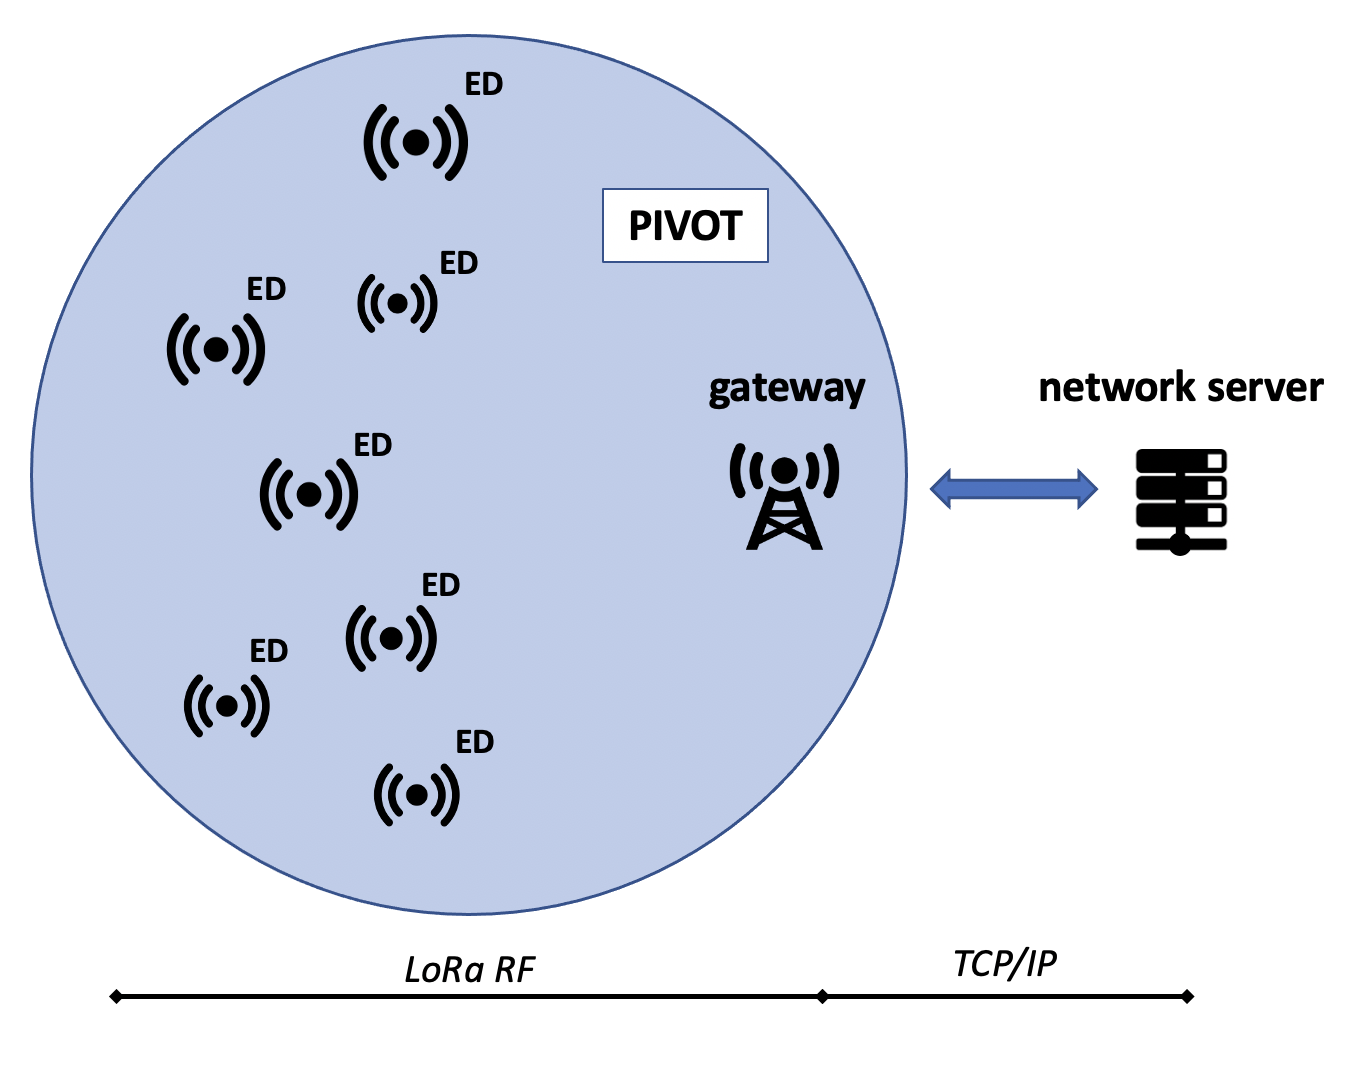
\includegraphics[width=0.7\linewidth]{images/pivot/architecture.png}
    \caption{The coverage area of PIVOT}
    \vspace{4ex}%
    \label{fig:coverage}
\end{figure}
As shown in Figure \ref{fig:coverage}, our system eavesdrops on the whole LoRa radio link area. Since symmetric key encryption is applied only to the payload, PIVOT has complete access to the text-clear header of the frames it collects. In particular, it requires the fields reported in Table \ref{tab:keys}.
\begin{table}[H]
    \vspace{4ex}%
    \caption{Key fields in the header, used by PIVOT}
    \label{tab:keys}
    \centering
    \begin{tabular}{|l|l|}
    \hline
        \textbf{PARAMETER} & \textbf{DESCRIPTION}                       \\ \hline
        DEV\_ADDR          & Unique identifier of the ED in the network \\ \hline
        DEV\_EUI           & Unique identifier of the physical ED       \\ \hline
	    FCnt		       & Frame counter                              \\ \hline
        TMST               & Internal clock timestamp                   \\ \hline
        TYPE               & Type of packet                             \\ \hline
    \end{tabular}
    \vspace{4ex}%
\end{table}
When the detection algorithm receives as input \textit{uplink} frame with a DevAddress \(\ a \) it has never seen before, checks which of the following two circumstances is met:
\begin{enumerate}
	\item The DevAddress \(\ a \) is linked to an ED that joins the network for the first time.
	\item The DevAddress \(\ a \) is linked to an ED, already in the network, that has disconnected and performed a new join procedure.
\end{enumerate}
When the second scenario occurs, PIVOT recognizes that the ED has a too predictable behavior, which could be the object of attack. It triggers the alert to the operator that, modifying the parameters of the device, can prevent it from being identified again.
\vspace{5mm}

\subsection{Patterns}
By hypothesis, each device has a transmission frequency, i.e. it regularly sends data to the server. Therefore, even when it disconnects from the network to then re-join it later, its behavior does not change. Formally, when an ED transmits packets periodically, we suppose it follows a temporal \textit{pattern} of period \(\tau\) that repeats continuously over time. Then, two DevAddress \(\ a_{1} \) and \(\ a_{2} \) which belongs to the same end-device, can be linked using a \textit{pattern-matching} strategy. 

\subsubsection{Notation}
PIVOT focuses on the time elapsed between an uplink message and the next one from the same endpoint.
In detail, let \(t_{i}\) the timestamp TMST of a packet \(p\) with a frame counter (FCnt) \(p_{fcnt} = i\), we define the \textit{segment} as the temporal distance between two consecutive messages with the same DevAddress (DEV\_ADDR):
\[\ s_{i} = t_{i+1} - t_{i} \]
Consequently, we define the pattern \(\ P \) of the device with DevAddress \(\ a \) as a \textit{chain} of segments.
\[\ P_{a} = \{ s_{1}, s_{2}, ... \}\]
The pattern has period \(\ \tau = s_{1} + ... + s_{n} \) where \(\ n \) is the number of segments in the chain of \(\ P \). 
\begin{figure}[H]
    \centering
    \vspace{4ex}%
    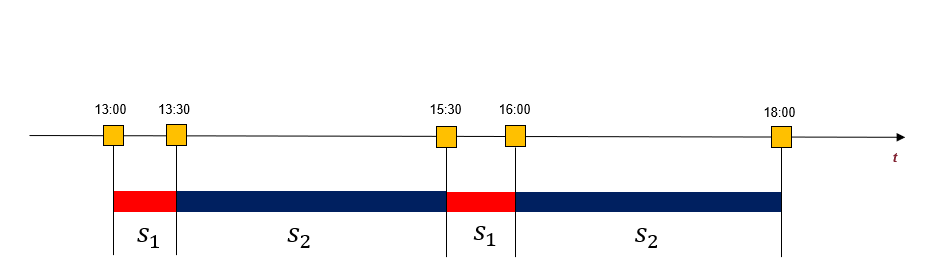
\includegraphics[width=0.7\linewidth]{images/pivot/pattern.PNG}
    \caption{An example of pattern \(\ P = \{ s_{1}, s_{2} \} \)}
    \vspace{4ex}%
    \label{fig:pattern}
\end{figure}
The Figure \ref{fig:pattern} reports an example of pattern \(\ P \). This end device sends uplink packets with the following frequency:
\begin{enumerate}
	\item Send the first packet of the sequence.
	\item Waits half an hour, then sends the second packet of the sequence.
	\item Waits two hours, then sends the third packet of the sequence.
	\item Repeat the sequence.
\end{enumerate}
Let \(\ s_{1} = 0.5 \) (half an hour) and \(\ s_{2} = 2.0 \) (two hours), then the device has the following pattern:
\[\ P = \{ s_{1}, s_{2} \} = \{ \textit{0.5}, \textit{2.0} \}\]
with period \(\ \tau = s_{1} + s_{2} = 2.5 \). In other words, this device repeats its pattern every two and a half hours.
\vspace{5mm}

\subsubsection{Building and updating patterns}
\label{updating}
PIVOT keeps track of every initialized pattern \(\ P \) by storing the following dynamic data:
\begin{itemize}
	\item The chain of segment \(\ \{ s_{1}, ..., s_{n} \} \) that composes the pattern \(\ P \).
	\item The current DevAddress \(\ a \) of the device.
	\item The timestamp \(\ t_{f} \) of the last packet sent by the device.
	\item A flag \textit{verified}, initially set to \texttt{False}.
\end{itemize}
For each new DevAddress \(\ a \), PIVOT initialize an \textit{empty} pattern \(\ P_{a} = \{\}\). The goal to fill the chain of \(\ P_{a} \), discovering the number and size of the segments that compose it. The last timestamp \(\ t_{f} \) received allow us to calculate the \textit{current} segment each time a new packet arrives and, if necessary, add it to the chain. 
\\
The \textit{verified} is a boolean flag that PIVOT sets to \textit{True} when it can estimate with a significantly high probability that the chain is complete. For example, the flag \(\ verified \) associate to the pattern \(\ P_{a} = \{ s_{1}, s_{2}, s_{3} \} \) is set to \textit{False} until the algorithm has correctly calculated all three segments of the chain.

\vspace{3mm}
\begin{figure}[H]
    \centering
    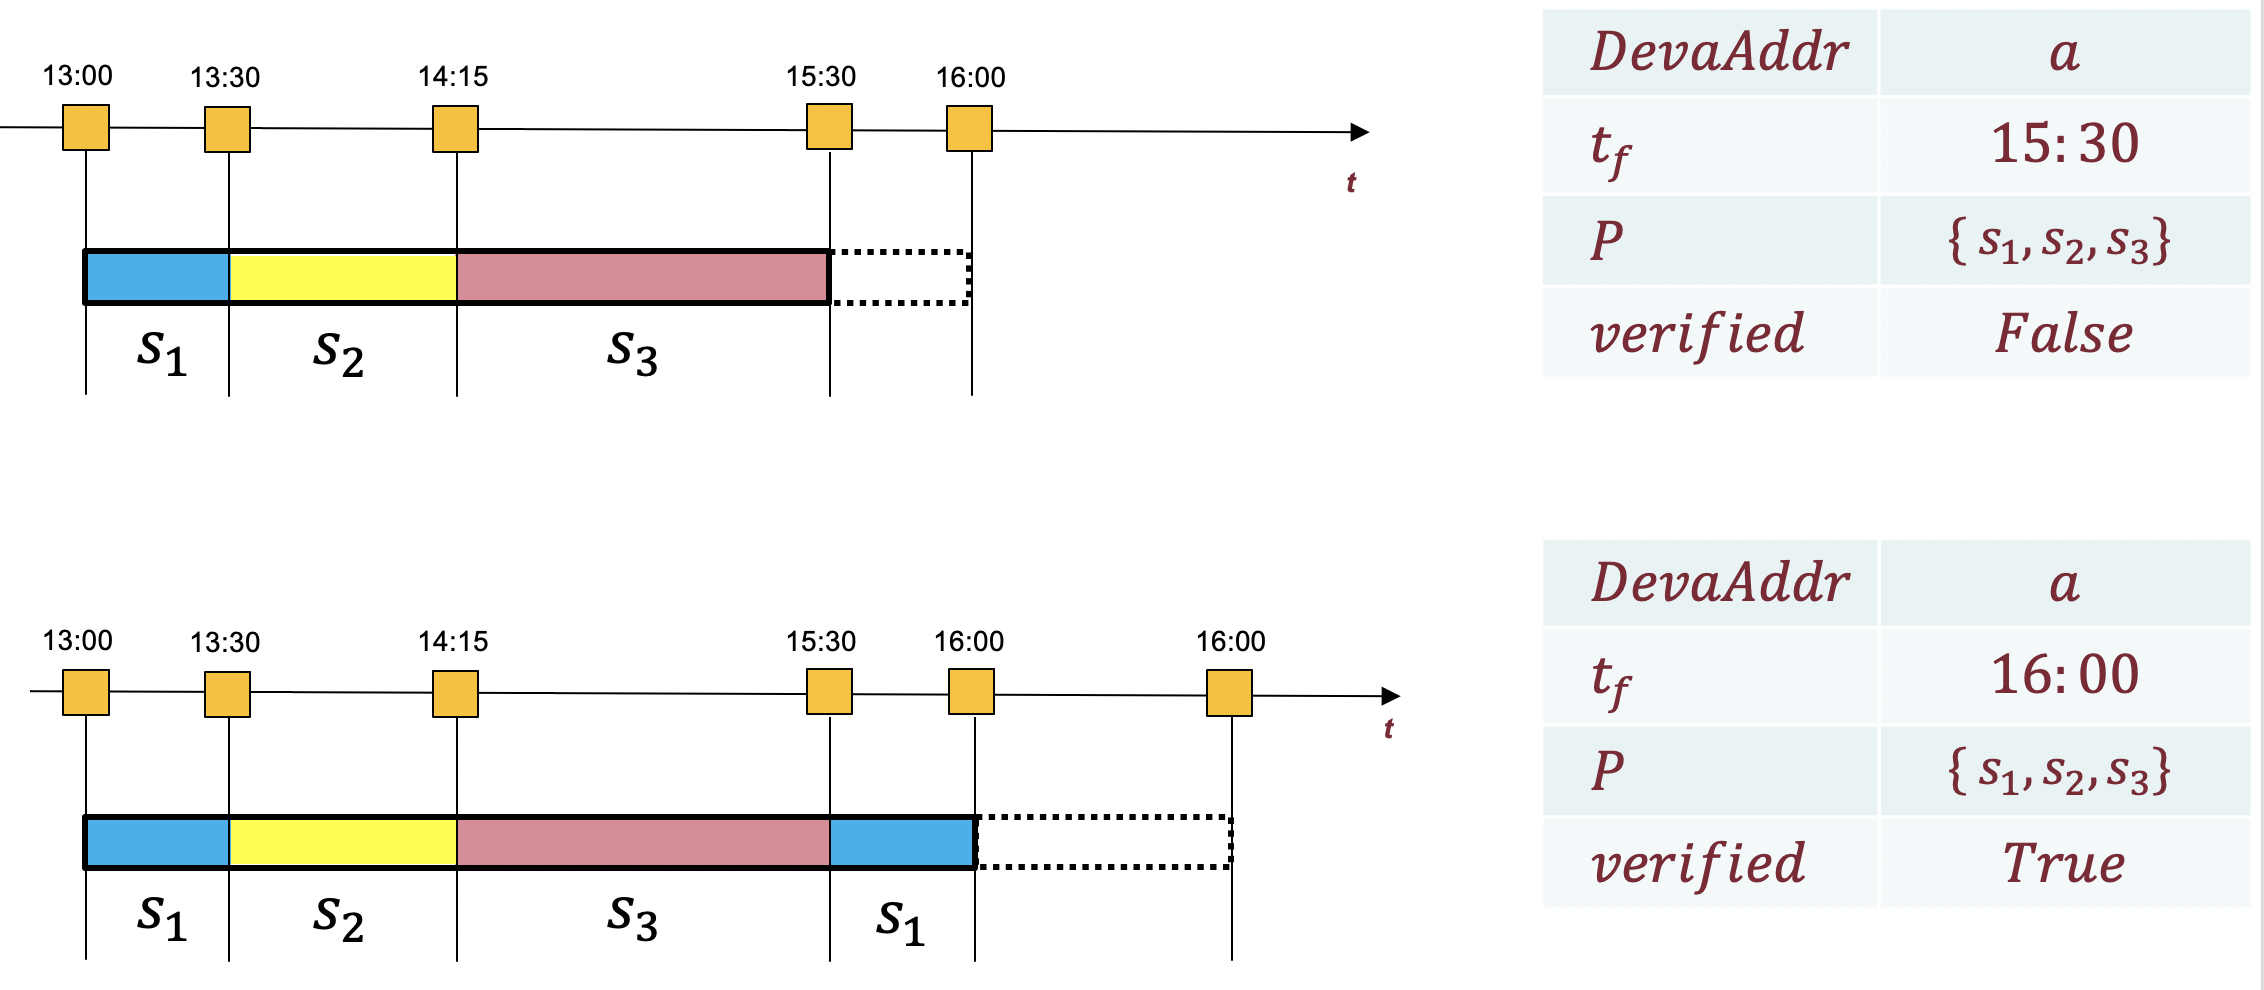
\includegraphics[width=0.7\linewidth]{images/pivot/updating.png}
    \caption{Updating of a pattern with a chain of three segments. After the update PIVOT changes only the parameters \(\ t_{f}\) and \(\ verified \). The chain don't change.}
    \label{fig:updating}
\end{figure}
\vspace{3mm}

When PIVOT receives a new packet \(\ p \) with DevAddress \(\ a \), it triggers the \textit{update} subroutine, reported with an example in figure \ref{fig:updating}. It works as follow:
\begin{enumerate}
	\item It calculates the \textit{current} segment \(\ s = t - t_{f} \), where \(\ t \) is the timestamp of \(\ p \) and \(\ t_{f} \) is the last timestamp associated to \(\ a \)
	\item It updates the last timestamp \(\ t_{f} = t \).
	\item It cheks if \(\ s \) is in the chain of \(\ P \). 
	\item It updates, if needed, the flag \(\ verified \).
\end{enumerate}
If detail, if the segment \(\ s \) in not in the chain, the subroutine add it to the bottom of the chain and sets the flag \(\ verified = False \).
On contrary, if the segment is already in the chain, PIVOT gets the flag \textit{verified} and, if it is currently set to \textit{False}, switch it to \textit{True}.

\vspace{3mm}
\begin{figure}[H]
    \centering
    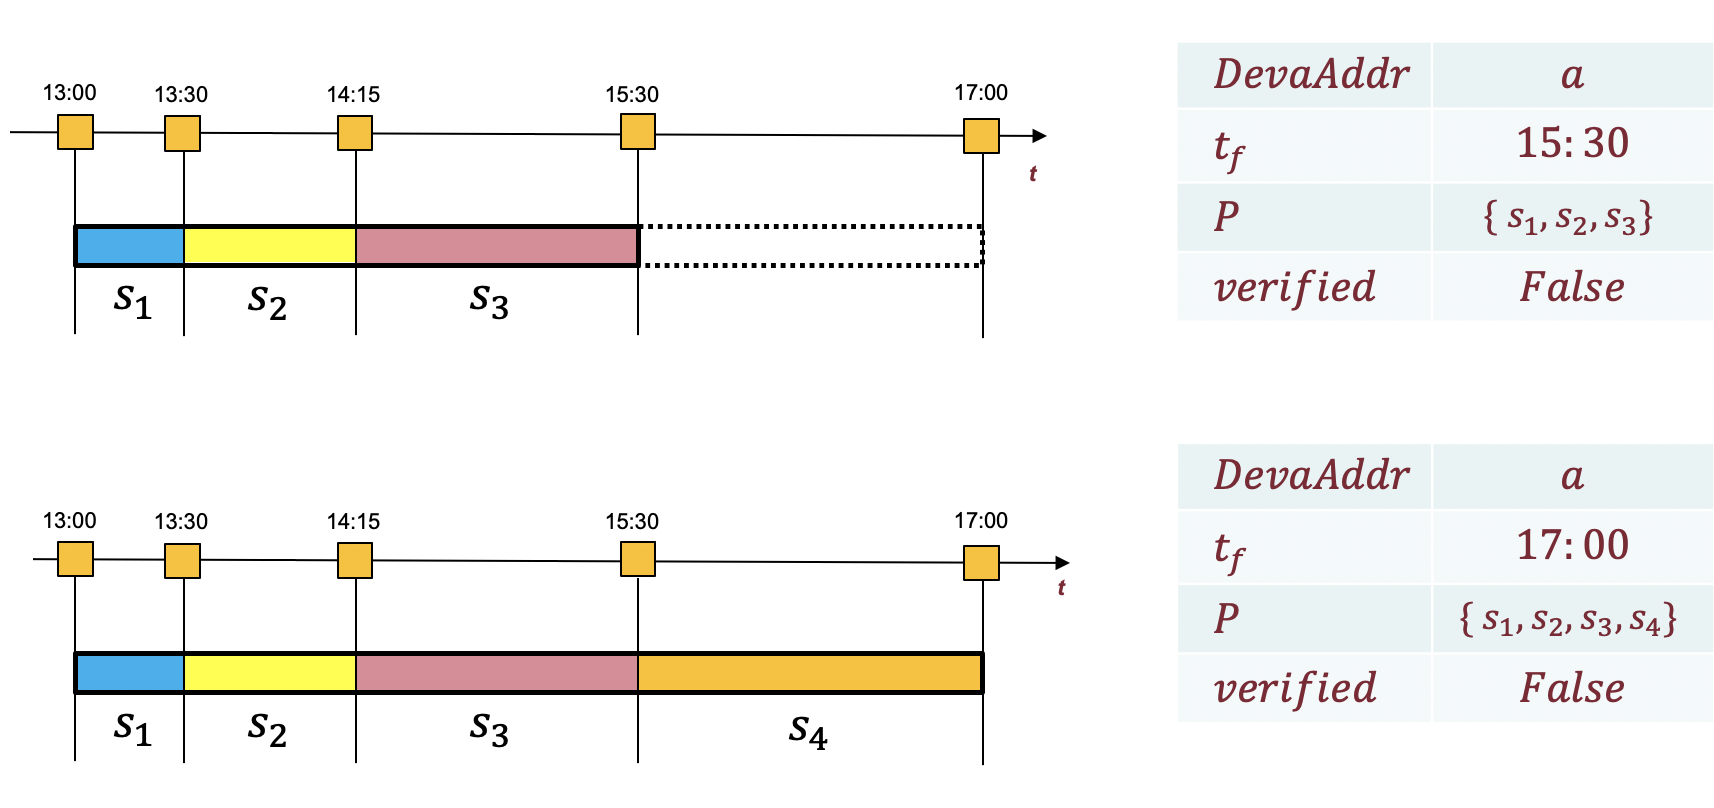
\includegraphics[width=0.7\linewidth]{images/pivot/updating_2.png}
    \caption{Updating of a pattern with a chain of four segments. After the update PIVOT changes the parameters \(\ t_{f}\) and append the new segment in the chain. The flag \(\ verified \) remains set to False.}
    \label{fig:updating_2}
\end{figure}
\vspace{3mm} %5mm vertical space

The figure \ref{fig:updating_2} shows an example in which the chain of \(\ P_{a} \) remains still incomplete after the update subroutine. Since the current segment was not present in the chain, it is appended at the bottom and the flag \textit{verified} remains set to \texttt{False}. Consequently, PIVOT cannot yet determine if this pattern is complete.
\vspace{5mm}

\subsubsection{Comparing the patterns}
Given two addresses \(\ a_{1} \) and \(\ a_{2} \) such that \(\ a_{1} \neq a_{2} \) and their patterns \(\ P_{a_{1}} \) and \(\ P_{a_{2}} \) such that \(\ P_{a_{1}} \equiv  P_{a_{2}} \). PIVOT concludes that \(\ P_{a_{1}} \) and \(\ P_{a_{2}} \) are \(\ equal \) and that \(\ a_{1} \) and \(\ a_{2}\) actually belong to the same device. This procedure is called \(\ matching\), and is the way the system identifies which devices are too exposed to external threats.
Two pattern \(\ P_{1} \) and \(\ P_{2} \) are equal when the following conditions are respected:
\begin{enumerate}
	\item The two chains are of the same length i.e. the patterns have the same period.
	\item The two chains are composed of the same number of segments.
	\item The two chains are composed of the same segments.
	\item the segments are \textit{sequentially} distributed in the same way within the chains.
\end{enumerate}
The figures \ref{fig:patterns_1} and \ref{fig:patterns_2} reports two examples where the pattern don't match.

\vspace{3mm}
\begin{figure}[H]
    \centering
    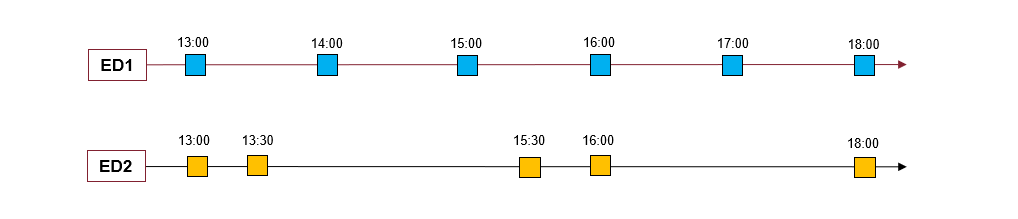
\includegraphics[width=0.7\linewidth]{images/pivot/patterns.PNG}
    \caption{Example of patterns with different period, number and type of segments.}
    \label{fig:patterns_1}
\end{figure}
\vspace{3mm}

In the first exmple, the pattern \(\ P_{1} \) consists of a single one-hour segment \(\ s_{1} = 1.0 \), the pattern \(\ P_{2} \) of two segments, one of 30 minutes \(\ s_{2} = 0.5 \) and one of 2 hours \(\ s_{3} = 2.0 \). PIVOT labels the two patterns \(\ P_{1} = \{s_{1}\} \) and \(\ P_{2} = \{s_{2}, s_{3}\} \) as different. First, they have two distinct periods \(\ \tau_{1} = 1.0 \) and \(\ \tau_{2} = 2.5 \). Second, the chains are composed by a diverse number and type of segments: the first chain one has one segment, the second one has two segments.

\vspace{3mm}
\begin{figure}[H]
    \centering
    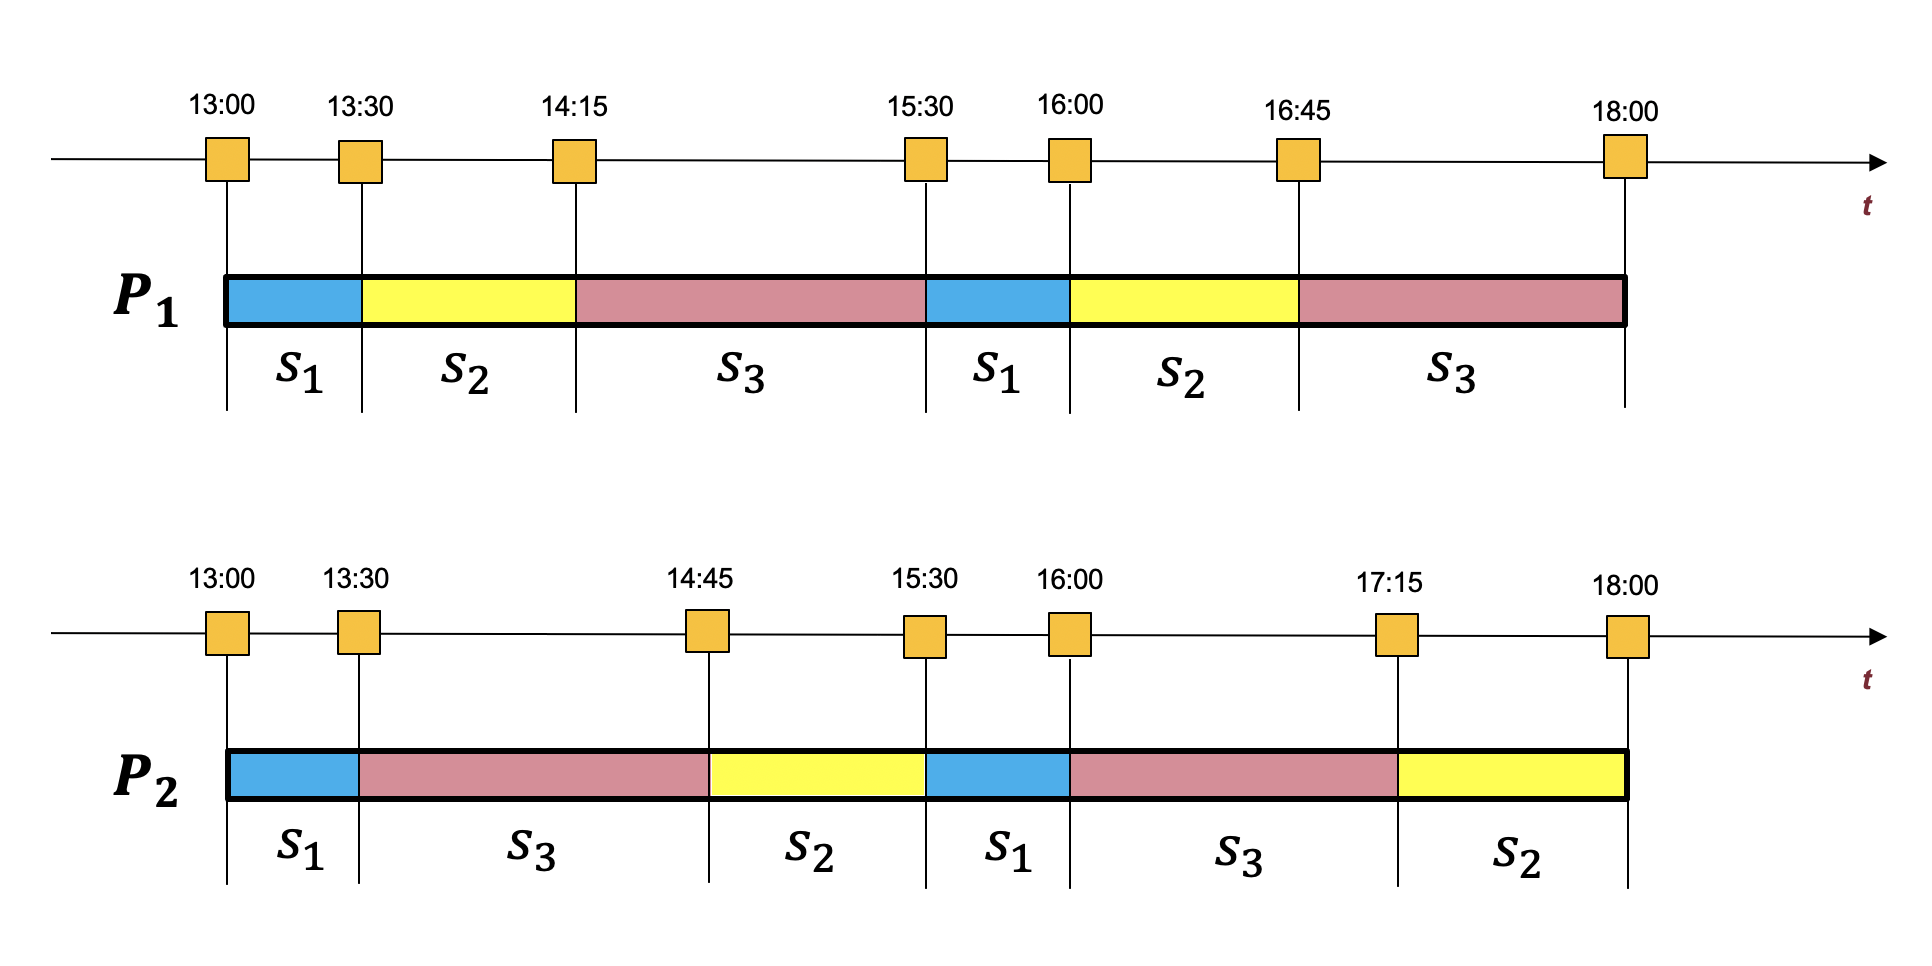
\includegraphics[width=0.7\linewidth]{images/pivot/patterns_2.PNG}
    \caption{Example of different patterns with the same period, number, and type of segments.}
    \label{fig:patterns_2}
\end{figure}
\vspace{3mm}

In the second example, the patterns have some common components, but they still don't match. Despite they have the same periods \(\ \tau_{1} = \tau_{2} = 2.5 \), the same number and the same type of segments \(\ s_{1}, s_{2}, s_{3} \), they are distributed differently in the two chains: \(\ P_{1} = \{ s_{1}, s_{2}, s_{3} \} \not\equiv P_{2} = \{ s_{1}, s_{3}, s_{2} \} \).
\vspace{5mm}

\subsection{Detection algorithm}
The purpose of the detection algorithm is to detect potentially too exposed devices. It analyzes the LoRa traffic, keeps track of all the detected DevAddress, and uses a pattern-matching strategy to verify if two collected DevAddress could be associated with the same ED.

\vspace{5mm}

In detail, the detection algorithm uses a vector \(\ C \) to store all the identified patterns. It contains a series of elements \(\ P_{a} \), where \(\ a \) is the current DevAddress associated to an ED, and \(\ P_{a} = \{ s_{1}, ..., s_{n} \} \) is the pattern the device follows. Since different patterns necessarily describe distinct EDs, in \(\ C \), there cannot be two tuples denoting the same device. In other words, let \(\ E \) be the set of all the ED that currently join the network, we have:
\[\ length(C) \subseteq length(E ) \]
The vector \(\ C \) allows checking if a given device, represented by its current DevAddres \(\ a \), already exchanged messages in the network. When the detection algorithm reads a new packet with DevAddress \(\ a \), it observe if the condition \(\ P_{a} \in C \) occurs. If \(\ P_{a} \notin C \) and this happens after the interception of a Join-request message, PIVOT  cannot establish \textit{a priori} the nature of the device associated to \(\ a \). It initiates a pattern-matching process to compute if \(\ a \) belongs to a new device or a re-joined one, trying to achieve this task in the shortest time possible. In this way, in the case of potential matching, the algorithm minimizes the delay in triggering the alert.

\vspace{5mm}

Intercepting a Join-request message is a crucial part of the detection process. It permits PIVOT to comprehend which addresses it needs to investigate and which patterns we should use for the matching procedure. The pattern \(\ P_{a} \notin C \), associated with an unknown address \(\ a \), should \textit{not} be compared with all the other patterns of \(\ C \). We must exclude from our analysis all that pattern related to these two classes of addresses:

\vspace{3mm}
\begin{itemize}
	\item All the addresses collected after the Join request, which have been noticed also before the Join-request. They are associated with devices that never disconnect from the network.
	\item All the other unknown addresses received after the Join-request, since a new device that joins the network has not more than one DevAddr.
\end{itemize}
\vspace{3mm}

The algorithm follows two sequential steps, called \textit{Pre-Join} procedure and \textit{Main} procedure. Figure \ref{fig:pre_main} illustrates the two procedures. Let \(\ t_{0} \) the timestamp of the first packet received by PIVOT after its activation and \(\ t_{f} \) the timestamp of the first Join-request packet. The Pre-Join procedure takes place in the time window \(\ t_{f} - t_{0} \) and the Main procedure starts after the reception of the first Join-Request message, at \(\ t_{f} \). In the next sections, we are going to examine these two steps in detail.

\begin{figure}[H]
    \centering
    \vspace{4mm}
    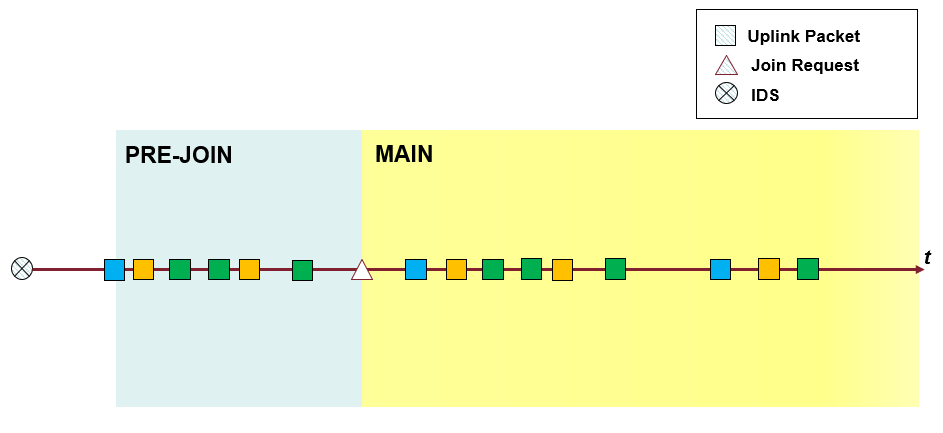
\includegraphics[width=0.7\linewidth]{images/pivot/pre-main.PNG}
    \caption{Representation of the time windows of the Pre-Join and Main procedures}
    \label{fig:pre_main}
\end{figure}
\vspace{5mm}

\begin{mintedbox}[samepage]{python}
def __pre_join(self, p):
    devaddr = p.dev_addr

    if devaddr in self.confirmed:
        self.confirmed[devaddr].update(p.t)
    else:
        self.confirmed[devaddr] = Pattern(p.t)
\end{mintedbox}
\subsubsection{Main procedure}
After the first Join-request message, the detection algorithm can no longer guarantee that a packet \(\ p \) with DevAddress \(\ a \) such that \(\ P_{a} \notin C \) necessarily belongs to a new, unregistered device. This time we have to consider also the hypothesis that the address \(\ a \) belongs to a  re-joined device. In detail, for each DevAddress \(\ a \), we have:

\vspace{3mm}
\begin{enumerate}
	\item \(\ P_{a} \in C \). \(\ a \) refers to a known ED, and it associated to a known pattern.
	\item \(\ P_{a} \notin C \). \(\ a \) refers to an unknown ED. The algorithm must recognize if it is belongs to a new device or an old one that re-joined the network.
\end{enumerate}
\vspace{3mm}

When the second scenario occurs, as in the Pre-Join procedure, a new pattern \(\ P_{a} \) is initialized. However, this time the pattern is not put in \(\ C \), but in a new vector, called \(\ U \), until the algorithm finds out if the address \(\ a \) represents a new device or not. Finally, the algorithm initialized the list \(\ TA_{a} \gets C \) of \textit{potential} patterns which could match with \(\ P_{a}\).

\vspace{5mm}

After the initialization of \(\ P_{a} \), each time the system receives as input a new packet \(\ p \) with the same address \(\ a \) and a new timestamp \(\ t \), the algorithm updates \(\ P_{a} \gets U \) and compares it with the patterns of \(\ TA_{a} \). Initially, the \(\ TA_{a} \gets verified(C) \) i.e. is it is composed of all the elements of C whose patterns is complete (then, with \textit{verified} flag set to \texttt{True}). After the updating of \(\ P_{a} \), three situations can occur:

\vspace{3mm}
\begin{enumerate}
	\item \(\ P_{a} \) doesn't match any element of \(\ TA_{a} \).
	\item The chain of \(\ P_{a} \) is a subset of one o more chains of the patterns of \(\ TA_{a} \).
	\item \(\ P_{a} \) matches \textit{exactly} with one o more elements of \(\ TA_{a} \).
\end{enumerate}
\vspace{3mm}

When the first scenario occurs, the DevAddress \(\ a \) necessarily represents a new ED. \(\ TA_{a} \) is erased from the storage and \(\ P_{a} \) is removed from \(\ U \) to be appended in \(\ C \). 

\vspace{5mm}

On the contrary, in the second case the chain of segments of \(\ P_{a} \) matches with the \textit{subchain} of one o more patterns of \(\ TA_{a} \). This implies that the chain of \(\ P_{a} \) may still be incomplete. Then the algorithm left \(\ P_{a} \) in the vector \(\ U \) and remove from \(\ TA_{a} \) all that pattern with which \(\ P_{a} \) don't match. 

\vspace{5mm}

In the last scenario, since there is a match between \(\ P_{a} \) and another pattern \(\ P_{b} \), most likely the associated addresses \(\ a \) and \(\ b \) belong to the same device. The algorithm inserts the \(\ P_{a} \) in a reservated vector, called \(\ Q \). When PIVOT will receive a new packet with DevAddress \(\ a \) such that \(\ P_{a} \in Q \), the algorithm starts the \textit{quarantine} subroutine, that will definitively confirm or reject the match between \(\ P_{a} \) and \(\ P_{b} \).

\vspace{3mm}
\begin{algorithm}
    \caption{Main procedure}
    \begin{algorithmic}[1]
        \If{$P_{a}$ n $C$}
            \State $P.update(t)$
        \Else
            \If{$P_{a}$ in $U$}
                \State $P.update(t)$
                \If{$P_{a}$ in $Q$}
                    \State quarantine procedure
                \EndIf
                \ForAll{$P_{ta}$ in $TA(a)$}
                    \If{$match(P_{a}, P_{ta})$}
                        \State $Q \gets P_{a}$
                    \Else
                        \State $TA(a).remove(P_{ta})$
                    \EndIf
                \EndFor
                \If{$TA(a)$ is empty}
                    \State new device
                    \State $C \gets P_{a}$
                \EndIf
            \Else
                \State $P \gets newPattern(a)$
                \State $U(a) \gets P$
                \State $TA(a) \gets verified(C)$
            \EndIf
        \EndIf
    \end{algorithmic}
\end{algorithm}

\newpage

\vspace{5mm}
\subsubsection{Quarantine}
\begin{figure}[t]
    \centering
    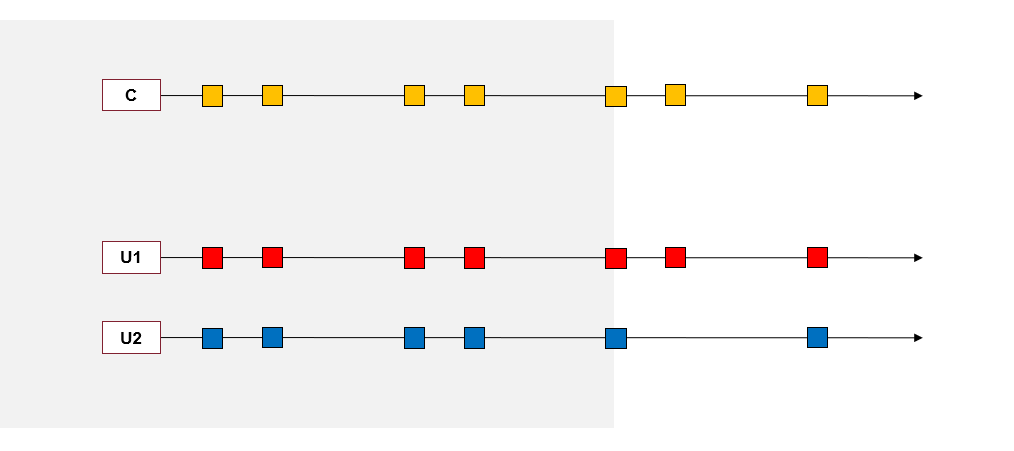
\includegraphics[width=0.7\linewidth]{images/pivot/quarantine.PNG}
    \caption{This example reports the two scenarios that can occur in the quarantine subroutine. In the first case, after updating the pattern \(\ U1 \), PIVOT confirms that \(\ U1 \) and \(\ C \) are linked to the same ED. In the second case, after updating the pattern \(\ U2 \), PIVOT confirms that \(\ U2 \) is associated to a new ED.}
    \label{fig:quarantine}
\end{figure}
When the incoming packet \(\ p \) has a DevAddress \(\ a \) such that \(\ P_{a} \in Q \), it means that \(\ P_{a} \) matches exactly with another pattern \(\ P_{b} \). The objective of the quarantine subroutine is to confirm this match or, on contrary, to demonstrate that \(\ P_{a} \) and \(\ P_{b} \) are linked to different EDs. Given the timestamp \(\ t \) of \(\ p \), the algorithm updates \(\ P_{a} \) and checks if \(\ P_{b} \) and \(\ P_{a} \) still match. If so, PIVOT triggers the \texttt{alert} the operator. If not, \(\ P_{a} \) belongs to a new device, then \(\ P_{a} \) moves from \(\ U \) to \(\ C \). The figure \ref{fig:quarantine} illustrates the two scenarios that can occur in the quarantine subroutine. Before of this step, the pattern \(\ C \) matches with both \(\ U1 \) and \(\ U2 \). In the first case, after updating \(\ U1 \) with the current timestamp \(\ t \), the algorithm confirms that \(\ U1 \) and \(\ C \) still matches. In the second case, after updating \(\ U2 \), the algorithm concluded that it represents the pattern of another device.

\vspace{3mm}
\begin{algorithm}[h!]
    \caption{Quarantine}
    \begin{algorithmic}[1]
        \State $P_{a} \gets U$
        \State $P_{b} \gets TA_{a}$
        \State $P_{a}.update(t)$
        \If{$match(P_{a}, P_{b})$}
            \State alert
        \Else
            \State new device
            \State $C \gets P_{a}$
        \EndIf
    \end{algorithmic}
\end{algorithm}
\vspace{5mm}

\newpage

\subsection{Metrics for operator}
PIVOT supports the network operator in its routine operations, providing a series of statistical metrics that illustrate the current state of the administered network.

\subsubsection{Number of Joins (NoJ)}
The Number of Joins (NoJ) represents the overall \textit{Join-request} messages intercepted and registered by PIVOT over the time. Generally, in LoRaWAN there is a \textit{peak} of Join-requests only in the starting phase when the operator registers and activates all the devices that will operate in the network. All Join-requests following this peak denote the insertion of new devices or the reconnection of old ones, two uncommon events. A too high value of NoJ might indicate the malfunction of one or more devices that are disconnecting and reconnecting continuously from the network. As demonstrated, sending a Join-request message could involve the expose the addresses of the device to unauthorized parties, then operator should avoid that the EDs send too many messages of this type.

\vspace{3mm}
\begin{figure}[H]
    \centering
    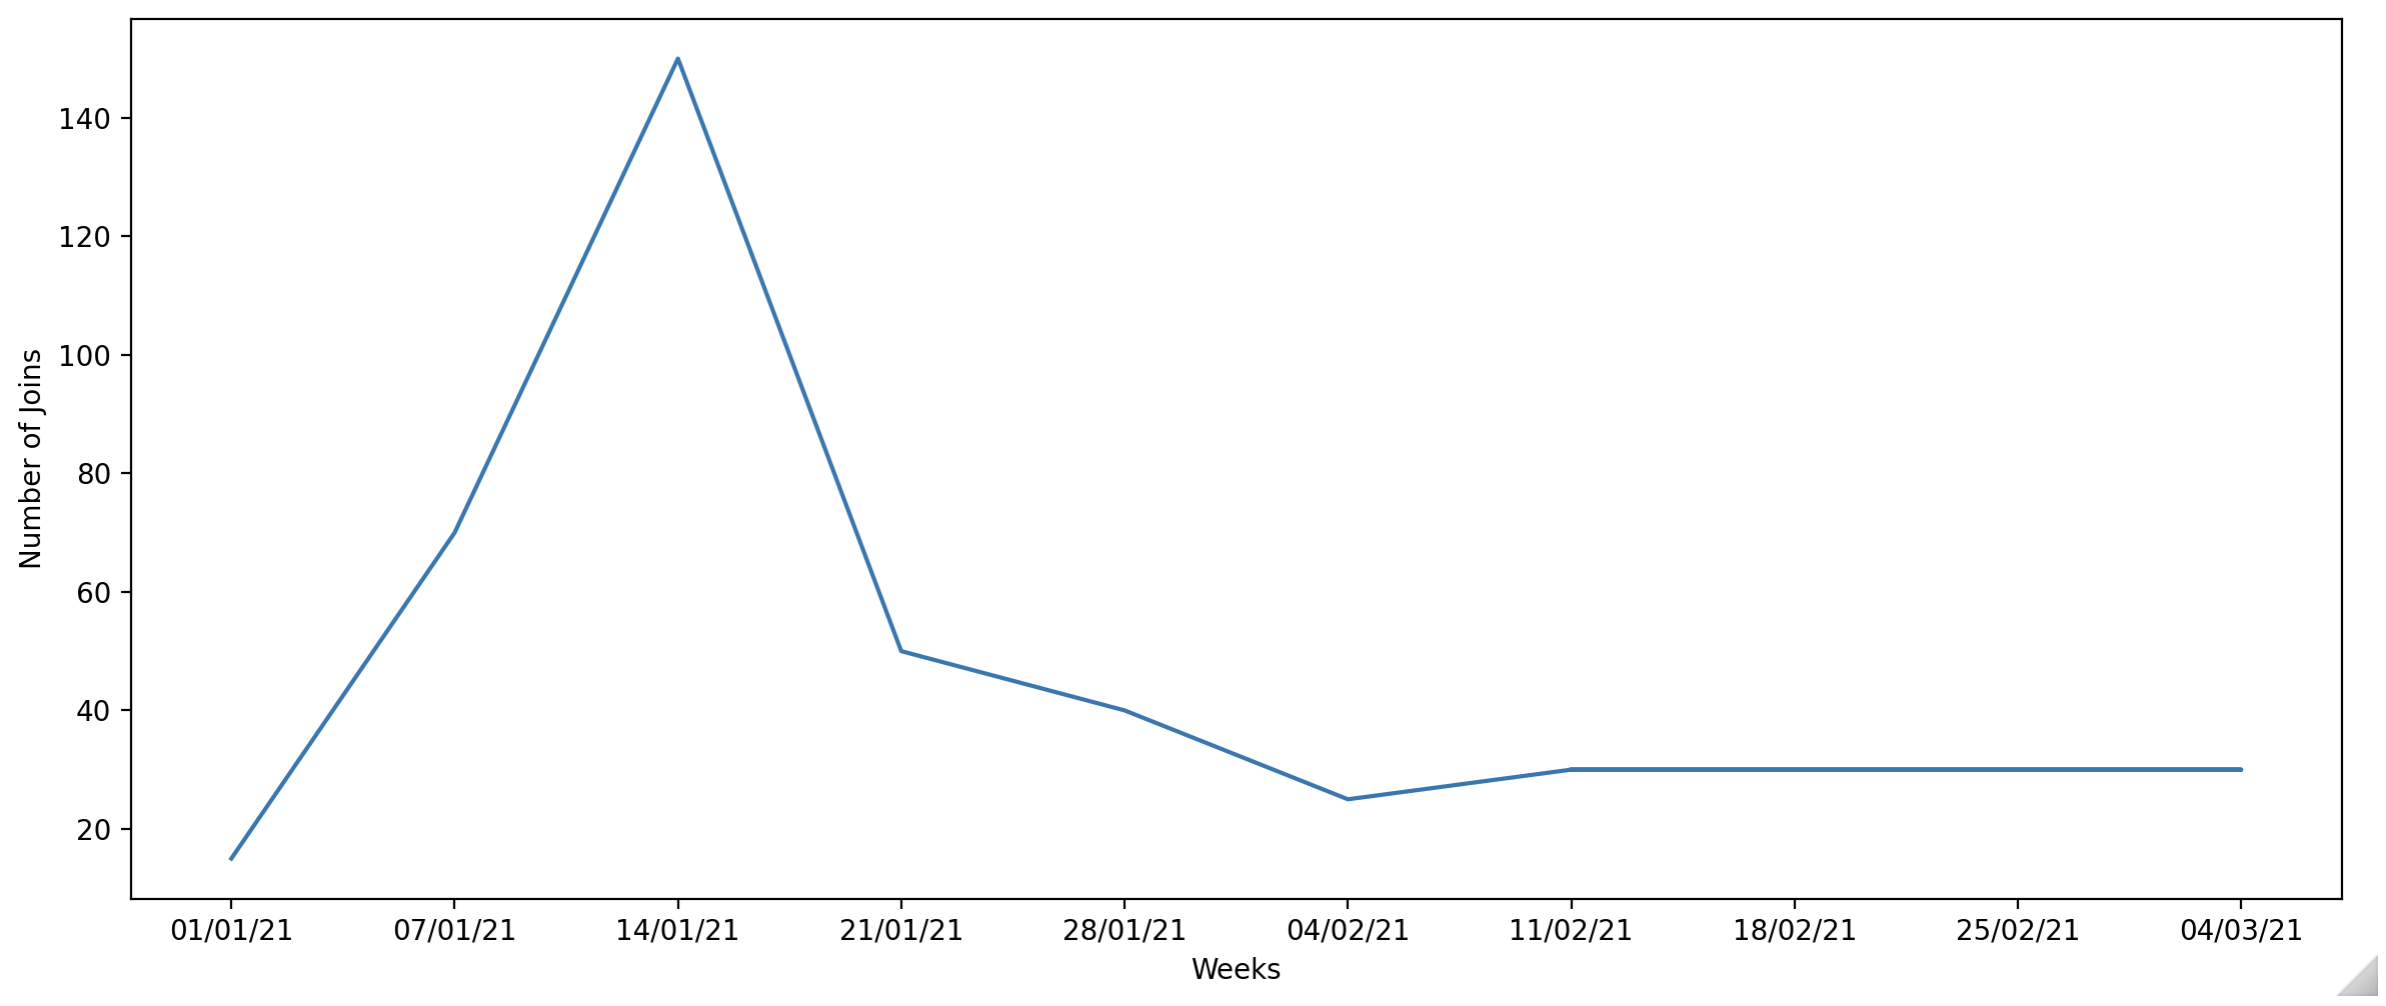
\includegraphics[width=0.7\linewidth]{images/pivot/NoJ.png}
    \caption{This plot reports an example of NoJ/weeks of a LoRaWAN network without anomaly devices. There is a peak only in the initial phase.}
    \label{fig:noj}
\end{figure}
\vspace{3mm}

\subsubsection{Number of Detected Devices (NoDD)}
The Number of Detected Devices (NoDD) describes the current amount of devices classified by PIVOT as vulnerable. These EDs, that re-joined the network at least once, have a too predictable pattern that could disclose their sensible characteristics, such as the identifiers, to external eavesdroppers. NoDD is updated each time PIVOT triggers the alert to the operator. This metric depends on the \textit{accuracy} of the detection algorithm of PIVOT, which may \textit{misclassify} some devices or miss capturing all vulnerable ones.

\subsubsection{Number of Unique Devices (NoUD)}
The Number of Unique Devices (NoUD) is the number of ED registered by PIVOT. These devices have sent at least one message to the server, exposing their DevAdress. NoUD does \textit{not} represent the total amount of devices of the network but only those that have transmitted packets since PIVOT was turned on. NoUD indicates the number of \textit{currently active} devices.

\subsubsection{Percentage of Detected Devices (PoDD)}
The Percentage of Detected Devices (PoDD) is a value in the range [0, 1] and represents the ratio between \textit{NoDD} and \textit{NoUD}. It provides a clear view of the network, showing exactly how many devices are vulnerable among all those present. Since it is not unusual for LoRa devices to generate periodic traffic, the PoDD value is generally always greater than zero. Using this metric, the operator can establish the \textit{maximum} permissible percentage of exposed devices, according to the dimension of the network. For example, in the case of environments made by a consistent number of devices, the management becomes more complex, and it is almost impossible to handle all the devices exposed. In this case, the goal could be to reduce the value of \textit{PoDD} whenever possible.